\documentclass[a4paper,twocolumn]{article}
\usepackage{lipsum}
\usepackage{marvosym}
\usepackage{graphicx}
\usepackage{subcaption}

\title{Introduction to \LaTeX}
\author{Meysam Shahbazi}

\begin{document}
\maketitle
\begin{abstract}
	
This is simple abstract.
next line 
	\lipsum[1]
	
\end{abstract}
\section{Introduction}
in ipsum in section \ref{sec:sub sub} we will use that.
\subsection{Lorum}
\lipsum[1]
\subsubsection{sub sub}\label{sec:sub sub}
\lipsum[1]
\paragraph{short point}
this is small point. 
\EUR


this is secntecs is still same part of paragraph

this is new paragraph
\subsection{Empesis}
\textbf{this is bold text} normal text.\textit{italic}
using very simple text .
\textbf{\textit{this is combine}}

{\tt this is sample type writter font.}
\subsection{Fonts size }
{\tiny this is tinny}  \\
\begin{normalsize}
this is normal text.
\end{normalsize} \\
\begin{huge}
	this is hugeee
\end{huge} \\
normal text
\subsection{Qoution}
normal text 

\begin{quote}
	ali said
	
\end{quote}

\subsection{figs}
in the figure \ref{figrue of cat} we see the cat \\
\lipsum

\begin{figure}
	
\includegraphics[width=\linewidth, angle=0,]{1_1_09_2f_37.png}
	\caption{my image caption}
	\label{figrue of cat} 
\end{figure}

\begin{figure*}
	
\includegraphics[width=\linewidth, angle=0,]{1_1_09_2f_37.png}
	\caption{my image caption}
	\label{figrue of big cat} 
\end{figure*}

\begin{figure}
	\begin{subfigure} {0.22\textwidth}
		
\includegraphics[width=\linewidth, angle=0,]{1_1_09_2f_37.png}
		\caption{my image caption 1}
		\label{fig gggggg}
		
	\end{subfigure}%
	\begin{subfigure} {0.22\textwidth}
		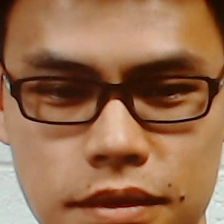
\includegraphics[width=\linewidth, angle=0,]{129-2-3-3-1f_385.png}
		\caption{my image caption}
		
	\end{subfigure}
	\caption{my figs}
\end{figure}

as seen in figure \ref{fig gggggg}


\lipsum
\section{table}
\lipsum
\begin{table}
	\centering
	\resizebox{0.5\textwidth}{!} {
	\begin{tabular} {l|cl}
		\hline
		col1 & col2 & col3 \\ \hline
		3 & 2 & 1 \\ \hline
		5 & 6 & 7 \\ \hline
		2 & 1 & 4 \\ \hline
		5 &  & 1 \\ \hline		
	\end{tabular}
}
\caption{ex table}
\end{table}


  
\end{document}